\documentclass[12pt]{article}
\usepackage[margin=0.75in]{geometry}
\usepackage{float}
\usepackage{multicol}
\usepackage{lmodern}
\usepackage{amssymb,amsmath}
\usepackage{ifxetex,ifluatex}
\usepackage{fixltx2e} % provides \textsubscript
\ifnum 0\ifxetex 1\fi\ifluatex 1\fi=0 % if pdftex
  \usepackage[T1]{fontenc}
  \usepackage[utf8]{inputenc}
\else % if luatex or xelatex
  \ifxetex
    \usepackage{mathspec}
    \usepackage{xltxtra,xunicode}
  \else
    \usepackage{fontspec}
  \fi
  \defaultfontfeatures{Mapping=tex-text,Scale=MatchLowercase}
  \newcommand{\euro}{€}
\fi
% use upquote if available, for straight quotes in verbatim environments
\IfFileExists{upquote.sty}{\usepackage{upquote}}{}
% use microtype if available
\IfFileExists{microtype.sty}{%
\usepackage{microtype}
\UseMicrotypeSet[protrusion]{basicmath} % disable protrusion for tt fonts
}{}
\usepackage{longtable,booktabs}
\usepackage{graphicx}
\makeatletter
\def\maxwidth{\ifdim\Gin@nat@width>\linewidth\linewidth\else\Gin@nat@width\fi}
\def\maxheight{\ifdim\Gin@nat@height>\textheight\textheight\else\Gin@nat@height\fi}
\makeatother
% Scale images if necessary, so that they will not overflow the page
% margins by default, and it is still possible to overwrite the defaults
% using explicit options in \includegraphics[width=3.5in][width, height, ...]{}
\setkeys{Gin}{width=\maxwidth,height=\maxheight,keepaspectratio}
\ifxetex
  \usepackage[setpagesize=false, % page size defined by xetex
              unicode=false, % unicode breaks when used with xetex
              xetex]{hyperref}
\else
  \usepackage[unicode=true]{hyperref}
\fi
\hypersetup{breaklinks=true,
            bookmarks=true,
            pdfauthor={Brandon LeBeau},
            pdftitle={PSQF 4143: Section 13},
            colorlinks=true,
            citecolor=blue,
            urlcolor=blue,
            linkcolor=magenta,
            pdfborder={0 0 0}}
\urlstyle{same}  % don't use monospace font for urls
\setlength{\parindent}{0pt}
\setlength{\parskip}{6pt plus 2pt minus 1pt}
\setlength{\emergencystretch}{3em}  % prevent overfull lines
\setcounter{secnumdepth}{0}

\title{PSQF 4143: Section 13}
\author{Brandon LeBeau}
\date{}

\begin{document}
\maketitle

\section{Dependent Groups}\label{dependent-groups}

\begin{itemize}
\itemsep1pt\parskip0pt\parsep0pt
\item
  Dependency between groups usually occurs in one of the following ways:

  \begin{enumerate}
  \def\labelenumi{\arabic{enumi}.}
  \itemsep1pt\parskip0pt\parsep0pt
  \item
    Repeated measures
  \item
    Matching
  \item
    Obtaining sets of identical twins or litter mates
  \item
    Obtaining pairs of participants who are matched by mutual selection
    (e.g.~husband-wife pairs, business partners).
  \end{enumerate}
\end{itemize}

\section{Exprimental Designs}\label{exprimental-designs}

\begin{enumerate}
\def\labelenumi{\arabic{enumi}.}
\itemsep1pt\parskip0pt\parsep0pt
\item
  Random Assignment (Independent Groups)
\item
  Matched Pairs (Dependent Groups)
\item
  Repeated Measures (Dependent Groups)
\end{enumerate}

\section{Random Assignment Example}\label{random-assignment-example}

\begin{itemize}
\itemsep1pt\parskip0pt\parsep0pt
\item
  Randomly select 50 UI freshmen
\item
  Randomly assign 25 to E-group and 25 to C-group
\item
  assuming the experiment is properly executed, with no biasing
  influences, the difference is due to

  \begin{itemize}
  \itemsep1pt\parskip0pt\parsep0pt
  \item
    chance factors associated with random assignment, and
  \item
    the treatment effect
  \end{itemize}
\end{itemize}

\section{Matched Pairs Example}\label{matched-pairs-example}

\begin{itemize}
\itemsep1pt\parskip0pt\parsep0pt
\item
  Randomly select 100 UI freshmen
\item
  Rank order by IQ
\item
  Form 50 matched pairs by randomly assigning one person from the first
  pair to E-group and the other to C-group, etc.
\item
  assuming the experiment is properly executed, with no biasing
  influences, the difference \(\bar{X}_{E} - \bar{X}_{C}\) is due to

  \begin{itemize}
  \itemsep1pt\parskip0pt\parsep0pt
  \item
    chance factors associated with random assignment, and
  \item
    the treatment effect, but
  \item
    not IQ, because it has been controlled for by matching
  \end{itemize}
\end{itemize}

\section{Repeated Measures Example}\label{repeated-measures-example}

\begin{itemize}
\itemsep1pt\parskip0pt\parsep0pt
\item
  Randomly select 50 UI freshmen
\item
  Administer pre-test
\item
  All participants take speed reading course
\item
  Administer post-test
\item
  Assuming no memory or practice effects associated with the pre-test,
  the difference \(\bar{X}_{post} - \bar{X}_{pre}\) is due to

  \begin{itemize}
  \itemsep1pt\parskip0pt\parsep0pt
  \item
    chance factors associated with random assignment, and
  \item
    the treatment effect, but
  \item
    not IQ, nor any other individual background characteristics, because
    they have been controlled for (each person serves as his/her own
    control)
  \end{itemize}
\end{itemize}

\section{Example 1}\label{example-1}

\begin{itemize}
\itemsep1pt\parskip0pt\parsep0pt
\item
  Does speed reading help or hurt reading comprehension?
\item
  Random sample of UI freshman students, n = 100
\item
  Students are rank ordered on ACT composite score
\item
  50 matched pairs of students are formed
\item
  One student from each pair is randomly assigned to the E-group, the
  other to the C-group
\item
  Experimental group (\(n_{E} = 50\)): speed reading course
\item
  Control group (\(n_{C} = 50\))
\end{itemize}

\section{Two ways to analyze}\label{two-ways-to-analyze}

\begin{itemize}
\itemsep1pt\parskip0pt\parsep0pt
\item
  There are two ways to analyze this data, the easy way and the hard
  way.

  \begin{itemize}
  \itemsep1pt\parskip0pt\parsep0pt
  \item
    The easy way we have seen before, the hard way is something
    completely new.
  \end{itemize}
\end{itemize}

\begin{longtable}[c]{@{}llll@{}}
\toprule
Pair & Experimental & Control & Difference\tabularnewline
\midrule
\endhead
1 & 38 & 36 & 2\tabularnewline
2 & 37 & 38 & -1\tabularnewline
. & . & . & .\tabularnewline
50 & 28 & 25 & 3\tabularnewline
\bottomrule
\end{longtable}

\begin{itemize}
\itemsep1pt\parskip0pt\parsep0pt
\item
  Easy Way:

  \begin{itemize}
  \itemsep1pt\parskip0pt\parsep0pt
  \item
    We take the mean and standard deviation of the difference scores
  \end{itemize}
\item
  Hard Way:

  \begin{itemize}
  \itemsep1pt\parskip0pt\parsep0pt
  \item
    Mean of both groups, standard deviations of both groups and the
    correlation between the two groups.
  \end{itemize}
\end{itemize}

\section{Example 1 (cont)}\label{example-1-cont}

\begin{itemize}
\itemsep1pt\parskip0pt\parsep0pt
\item
  Suppose:

  \begin{itemize}
  \itemsep1pt\parskip0pt\parsep0pt
  \item
    \(\bar{D} = 4\)
  \item
    \(S_{D} = 7\)
  \end{itemize}
\item
  Is \(\bar{D} = 4\) an unlikely outcome?
\item
  We need a probability distribution for \(\bar{D}\).
\end{itemize}

\section{Sampling Distribution of difference
scores}\label{sampling-distribution-of-difference-scores}

\begin{figure}[H]
\centering
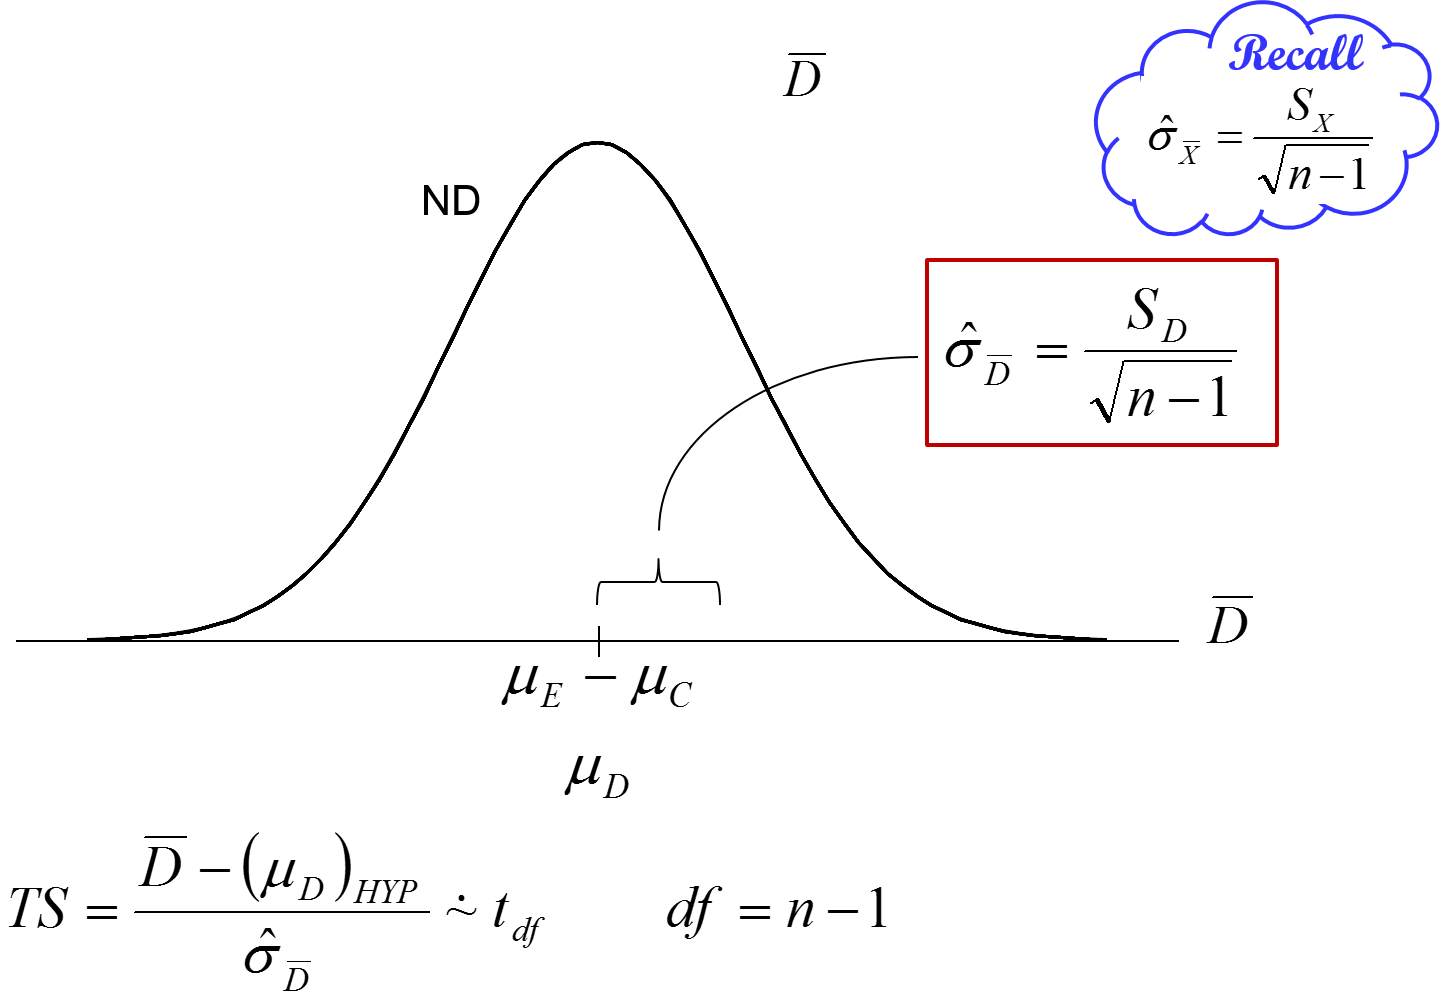
\includegraphics[width=3.5in]{samp_dist_diff.png}
\caption{}
\end{figure}

\section{Example 2}\label{example-2}

\begin{figure}[H]
\centering
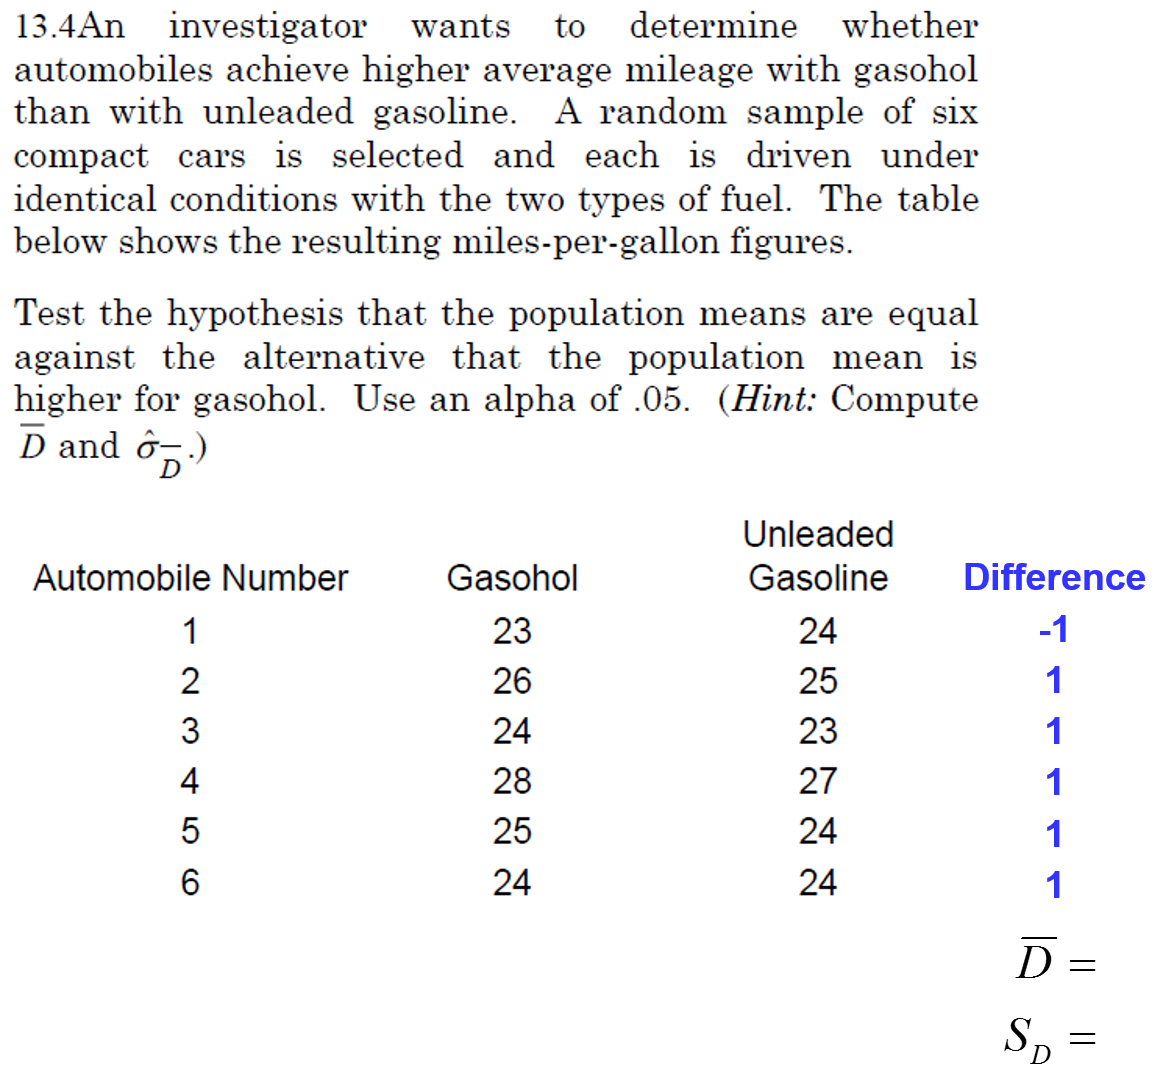
\includegraphics[width=3.5in]{dep_ttest_example2.png}
\caption{}
\end{figure}

\section{Standard Error Hard Way}\label{standard-error-hard-way}

\begin{figure}[H]
\centering
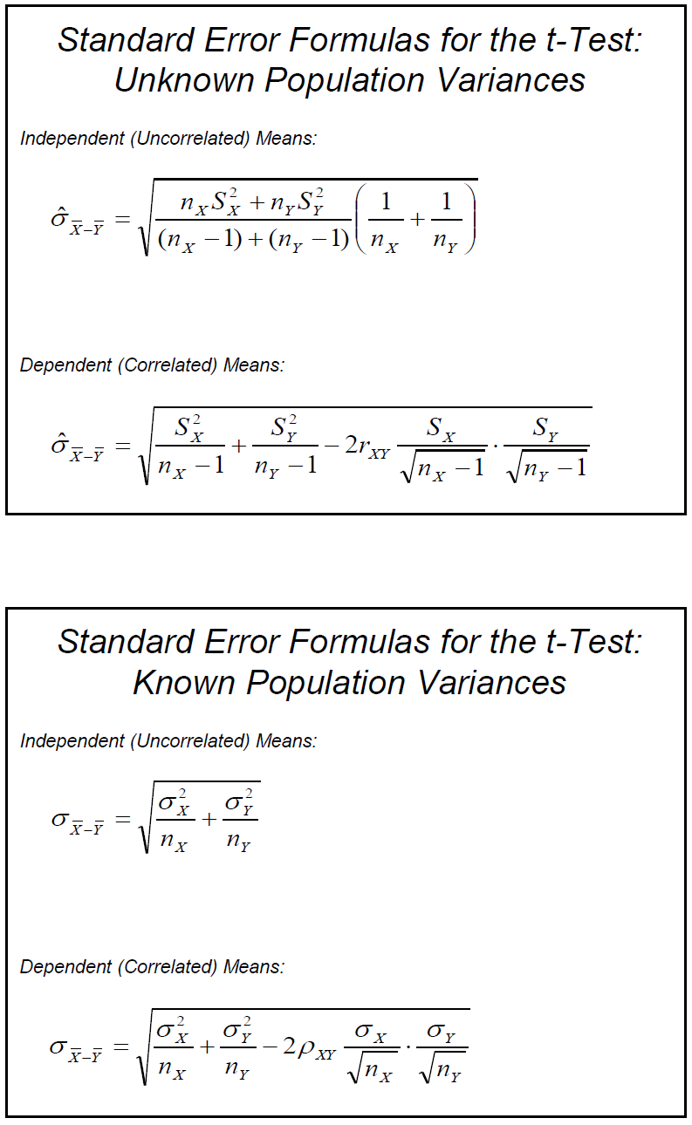
\includegraphics[width=3.5in]{dep_se_hardway.png}
\caption{}
\end{figure}

\section{Standard Error Hard Way 2}\label{standard-error-hard-way-2}

\begin{itemize}
\item
  Independent (uncorrelated) means:
  \[ \sigma_{\bar{X} - \bar{Y}} = \sqrt{\frac{\sigma_{X}^{2}}{n_{X}} + \frac{\sigma_{Y}^{2}}{n_{Y}}} \]
\item
  Dependent (correlated) means:
  \[ \sigma_{\bar{X} - \bar{Y}} = \sqrt{\frac{\sigma_{X}^{2}}{n_{X}} + \frac{\sigma_{Y}^{2}}{n_{Y}} - 2 \rho_{XY} \frac{\sigma_{X}}{\sqrt{n_{X}}} \frac{\sigma_{Y}}{\sqrt{n_{Y}}}} \]
\item
  When \(\rho = 0\), \(SE_{dep} = SE_{ind}\)
\item
  When \(\rho > 0\), \(SE_{dep} < SE_{ind}\)
\item
  When \(\rho < 0\), \(SE_{dep} > SE_{ind}\)
\end{itemize}

\section{Advantages of dependent means
design}\label{advantages-of-dependent-means-design}

\begin{itemize}
\itemsep1pt\parskip0pt\parsep0pt
\item
  Repeated measures or pairing of observations makes possible the
  elimination of an extraneous source of variation
\item
  The reduction in standard error that is induced by pairing the
  observations depends on the value of \(\rho_{XY}\) (population
  correlation between X and Y)
\item
  so how do we know whether \(\rho_{XY}\) is 0 , + , or -- ?

  \begin{itemize}
  \itemsep1pt\parskip0pt\parsep0pt
  \item
    when the matching variable is positively related to the outcome of
    interest, \(\rho_{XY}\) is positive
  \item
    when the matching variable is negatively related to the outcome of
    interest, \(\rho_{XY}\) is negative
  \end{itemize}
\end{itemize}

\section{Advantages of dependent means design
2}\label{advantages-of-dependent-means-design-2}

\begin{itemize}
\itemsep1pt\parskip0pt\parsep0pt
\item
  When pairing is on the basis of a variable that is positively and
  importantly related to the performance of the participants on the
  outcome variable, \(\rho_{XY}\) will be higher than otherwise

  \begin{itemize}
  \itemsep1pt\parskip0pt\parsep0pt
  \item
    consequently, the reduction in the standard error will be greater
  \item
    decreased standard error results in increased power
  \end{itemize}
\end{itemize}

\section{Advantages of dependent means design
3}\label{advantages-of-dependent-means-design-3}

\begin{itemize}
\itemsep1pt\parskip0pt\parsep0pt
\item
  However, note that pairing of observations cuts the df in half

  \begin{itemize}
  \itemsep1pt\parskip0pt\parsep0pt
  \item
    smaller df results in decreased power
  \item
    the smaller the df, the thicker the tails of the t-distribution
  \item
    and the further out in the tails the critical region
  \item
    this effect is especially pronounced when sample size is small
    (\(n < 50\))
  \end{itemize}
\item
  Thus, \(\rho_{XY}\) must be large enough to offset the decrease in
  power, induced by the lower df which results from pairing
\end{itemize}

\section{Assumptions}\label{assumptions}

\begin{itemize}
\itemsep1pt\parskip0pt\parsep0pt
\item
  In testing \(H_{0}: \mu_{D} = 0\), it is assumed that the population
  of differences (\(D = X - Y\)) is normally distributed

  \begin{itemize}
  \itemsep1pt\parskip0pt\parsep0pt
  \item
    These differences will be normally distributed if X and Y are
    normally distributed
  \end{itemize}
\item
  If repeated measures are obtained, it is assumed that participants are
  a random sample from the population of interest

  \begin{itemize}
  \itemsep1pt\parskip0pt\parsep0pt
  \item
    The order in which the conditions are presented should be randomized
    for each participant if the nature of the independent variable
    permits it
  \end{itemize}
\item
  If pairs of matched participants are used, the participants in each
  pair should be randomly assigned to experimental and control
  conditions
\end{itemize}

\section{Calculating a confidence
interval}\label{calculating-a-confidence-interval}

\begin{itemize}
\itemsep1pt\parskip0pt\parsep0pt
\item
  Recall speed reading data

  \begin{itemize}
  \itemsep1pt\parskip0pt\parsep0pt
  \item
    \(n = 50\); \(\bar{D} = 4\); \(S_{D} = 7\)
  \end{itemize}
\item
  Suppose we wanted to calculate a 99\% CI for \(\mu_{D}\)
\item
  We can do that with the following form:
  \[ \bar{X}_{D} \pm t_{crit} * \frac{S_{D}}{\sqrt{n - 1}} \]
\end{itemize}

\section{Interpreting a confidence
interval}\label{interpreting-a-confidence-interval}

\begin{itemize}
\itemsep1pt\parskip0pt\parsep0pt
\item
  Interpretations for 99\% CI {[}1.32, 6.68{]}:

  \begin{enumerate}
  \def\labelenumi{\arabic{enumi}.}
  \itemsep1pt\parskip0pt\parsep0pt
  \item
    Does \(\mu_{D}\) fall in this interval?
  \item
    Is there a 99\% chance that \(\mu_{D}\) falls in this interval?
  \item
    If 100 intervals were constructed, about how many intervals would
    contain \(\mu_{D}\)?
  \item
    If we constructed an infinte number of intervals, how many would
    contain \(\mu_{D}\)?
  \end{enumerate}
\end{itemize}

\section{Using confidence intervals to conduct a two-tailed
hypothesis}\label{using-confidence-intervals-to-conduct-a-two-tailed-hypothesis}

\begin{itemize}
\itemsep1pt\parskip0pt\parsep0pt
\item
  You can use a confidence interval to conduct a two-tailed hypothesis
  of any null hypothesis.

  \begin{itemize}
  \itemsep1pt\parskip0pt\parsep0pt
  \item
    If the hypothesized value falls within the CI, fail to reject
    \(H_{0}\)
  \item
    If the hypothesized value falls outside the CI, reject \(H_{0}\)
  \end{itemize}
\item
  Using the previous example {[}1.32, 6.68{]}, would we fail to reject
  or reject \(H_{0}\)?
\end{itemize}

\section{Three Experimental Designs}\label{three-experimental-designs}

\begin{enumerate}
\def\labelenumi{\arabic{enumi}.}
\itemsep1pt\parskip0pt\parsep0pt
\item
  Random Assignment (Independent Groups)

  \begin{itemize}
  \itemsep1pt\parskip0pt\parsep0pt
  \item
    Randomly select 50 UI freshmen
  \item
    Randomly assign 25 to E-group and 25 to C-group
  \end{itemize}
\item
  Matched Pairs (Dependent Groups)

  \begin{itemize}
  \itemsep1pt\parskip0pt\parsep0pt
  \item
    Randomly select 100 UI freshmen
  \item
    Rank order by IQ
  \item
    Randomly assign one person from the first pair to E-group and the
    other to C-group, etc.
  \end{itemize}
\item
  Repeated Measures (Dependent Groups)

  \begin{itemize}
  \itemsep1pt\parskip0pt\parsep0pt
  \item
    Randomly select 50 UI freshmen
  \item
    Administer pre-test
  \item
    All participants take speed reading course
  \item
    Administer post-test
  \end{itemize}
\end{enumerate}

\end{document}
